% -----------------------------------------------
% Template for SMAC SMC 2013
% adapted and corrected from the template for SMC 2012, which was adapted from that of SMC 2011
% further updated for TENOR 2015, 2016, 2017 and 2018
% -----------------------------------------------

\documentclass{article}
\usepackage{tenor}
\usepackage{ifpdf}
\usepackage[english]{babel}
\usepackage{balance}

%%%%%%%%%%%%%%%%%%%%%%%% Some useful packages %%%%%%%%%%%%%%%%%%%%%%%%%%%%%%%
%%%%%%%%%%%%%%%%%%%%%%%% See related documentation %%%%%%%%%%%%%%%%%%%%%%%%%%
%\usepackage{amsmath} % popular packages from Am. Math. Soc. Please use the 
%\usepackage{amssymb} % related math environments (split, subequation, cases,
%\usepackage{amsfonts}% multline, etc.)
%\usepackage{bm}      % Bold Math package, defines the command \bf{}
%\usepackage{paralist}% extended list environments
%%subfig.sty is the modern replacement for subfigure.sty. However, subfig.sty 
%%requires and automatically loads caption.sty which overrides class handling 
%%of captions. To prevent this problem, preload caption.sty with caption=false 
%\usepackage[caption=false]{caption}
%\usepackage[font=footnotesize]{subfig}


% REDEFINE THESE VARIABLES:
\def\papertitle{PAPER TEMPLATE FOR TENOR}
\def\firstauthor{First author}
\def\secondauthor{Second author}
\def\thirdauthor{Third author}

\def\copyrightyear{2022}

%% Depending on the number of authors, set this vriable accordingly for the copyright notice:
% \def\copyrightauthors{Author One}
\def\copyrightauthors{Author One and Author Two}
% \def\copyrightauthors{Author One, Author Two et al}

% adds the automatic
% Saves a lot of ouptut space in PDF... after conversion with the distiller
% Delete if you cannot get PS fonts working on your system.

% pdf-tex settings: detect automatically if run by latex or pdflatex
\newif\ifpdf
\ifx\pdfoutput\relax
\else
   \ifcase\pdfoutput
      \pdffalse
   \else
      \pdftrue
\fi

\ifpdf % compiling with pdflatex
  \usepackage[pdftex,
    pdftitle={\papertitle},
    pdfauthor={\firstauthor},
    bookmarksnumbered, % use section numbers with bookmarks
    pdfstartview=XYZ % start with zoom=100% instead of full screen; 
                     % especially useful if working with a big screen :-)
   ]{hyperref}
  %\pdfcompresslevel=9

  \usepackage[pdftex]{graphicx}
  % declare the path(s) where your graphic files are and their extensions so 
  %you won't have to specify these with every instance of \includegraphics
  \graphicspath{{./figures/}}
  \DeclareGraphicsExtensions{.pdf,.jpeg,.png}

  \usepackage[figure,table]{hypcap}

\else % compiling with latex
  \usepackage[dvips,
    bookmarksnumbered, % use section numbers with bookmarks
    pdfstartview=XYZ % start with zoom=100% instead of full screen
  ]{hyperref}  % hyperrefs are active in the pdf file after conversion

  \usepackage[dvips]{epsfig,graphicx}
  % declare the path(s) where your graphic files are and their extensions so 
  %you won't have to specify these with every instance of \includegraphics
  \graphicspath{{./figures/}}
  \DeclareGraphicsExtensions{.eps}

  \usepackage[figure,table]{hypcap}
\fi

%setup the hyperref package - make the links black without a surrounding frame
\hypersetup{
    colorlinks,%
    citecolor=black,%
    filecolor=black,%
    linkcolor=black,%
    urlcolor=black
}


% Title.
% ------
\title{\papertitle}

% Authors
% Please note that submissions are NOT anonymous, therefore 
% authors' names have to be VISIBLE in your manuscript. 
%
% Single address
% To use with only one author or several with the same address
% ---------------
\oneauthor
   {\firstauthor} {Affiliation \\ City, Country \\
     {\tt \href{mailto:author1@adomain.org}{author1@adomain.org}}}

%Two addresses
%--------------
% \twoauthors
%   {\firstauthor} {Affiliation \\ City, Country \\ 
%     {\tt \href{mailto:author1@adomain.org}{author1@adomain.org}}}
%   {\secondauthor} {Affiliation \\ City, Country \\ 
%     {\tt \href{mailto:author2@adomain.org}{author2@adomain.org}}}

% Three addresses
% --------------
% \threeauthors
%   {\firstauthor} {Affiliation \\ City, Country \\ 
%     {\tt \href{mailto:author1@adomain.org}{author1@adomain.org}}}
%   {\secondauthor} {Affiliation \\ City, Country \\ 
%     {\tt \href{mailto:author2@adomain.org}{author2@adomain.org}}}
%   {\thirdauthor} { Affiliation \\ City, Country \\ 
%     {\tt \href{mailto:author3@adomain.org}{author3@adomain.org}}}


% ***************************************** the document starts here ***************
\begin{document}
%
\capstartfalse
\maketitle
\capstarttrue
%
\begin{abstract}
The abstract should placed at the top left column on the first page. 
Please write about 150-200 words that specifically highlight the purpose of your work, its context, and provide a brief synopsis of your results. 
Abstract should be one single paragraph and not contain equations, special characters or specific format instructions (bullet lists, URLs, etc.) 
Do not use citations or footnotes in the abstract. 
As all first paragraphs, the abstract should not be indented.
\end{abstract}
%

\section{Introduction}\label{sec:introduction}
This template includes the information about formatting manuscripts for the TENOR conference.
Please follow these guidelines carefully.
The \textbf{tenor.sty} file provided in the \LaTeX{} templates should make the most of it automatically.
If you prepare your document by cutting and pasting into this one, then you should not have to worry, 
unless there is something strange with your \LaTeX{} interpreter.
If you have any questions, please contact the conference organizers.

\section{Page size and format}\label{sec:page_size}
The proceedings will be formatted as portrait A4-size paper (21.0~cm x 29.7~cm).
All material on each page should fit within a rectangle of 17.2~cm x 25.2~cm, centered on the page, beginning 2.0~cm from the top of the page and ending with 2.5cm from the bottom.
The left and right margins should be 1.9~cm.
The text should be in two 8.2~cm columns with a 0.8~cm gutter.
All text must be in a two-column format, and justified.

The maximum allowed length is 10 pages. 
We encourage a paper length of 6-8 pages.

\section{Copyright Notice}\label{sec:copyright}

Do not move the copyright notice from his original position, as defined by the \textbf{tenor.sty} file (i.e. at the bottom of the first column). 

Fill in the year and author names by redefining the variables \texttt{copyrightyear} and \texttt{copyrightauthor} in the heading part of the template .tex file.

\section{Typeset Text}\label{sec:typeset_text}

\subsection{Normal or Body Text}\label{subsec:body}
Please use a 10pt (point) Times font. 
Sans-serif or non-proportional fonts can be used only for special purposes, such as distinguishing source code from text.

The first paragraph in each section should not be in-dented, but all other paragraphs should be (0,25cm). Line should be single spaced. Avoid orphan lines, and do not break columns manually (leave the text down to the bottom of the columns). Do not leave blank lines or space between paragraphs. Use non-breakable space to avoid line breaks just before figure, numbers, references, etc. 

Use ``curly quotes'', \textit{italics} but avoid other formatting effects if possible. 
URL text color must remain black.

\subsection{Title and Authors}

As you can see above, the title is 14pt Times, bold, upper case, and centered.
The names of the authors are also bold and centered.
Just use and follo instructions in this template .tex file.
The lead author's name is to be listed first (left-most), and the co-authors' 
names after. 
If the addresses for all authors are the same, include the 
address only once, centered. If the authors have different addresses, put the 
addresses, evenly spaced, under each authors' name.


\subsection{Lists}

Below is the preferred format for bullet and numbered list.

\begin{itemize}\itemsep0pt % use \itemsep if necessary to reduce space between items
\item One item (note the bullet symbol used o).
\item Another item spreading over several lines (beware of indentation and spacing).
\item Sub-lists are discouraged but authors are free to choose the symbol for it.
\end{itemize}

\begin{enumerate}\itemsep0pt
\item A numbered item
\item Another numbered item spreading on several lines of text.
\end{enumerate}


\subsection{Page Numbering, Headers and Footers}

Do not include headers, footers or page numbers in your submission. 
These will be added electronically at a later stage, when the publications are assembled.

\section{Headings}

First level headings are in Times 10pt bold, centered.

\subsection{Second Level Headings}

Second level headings are in Times 10pt bold, flush left.
The first letter of each significant word is capitalized.

\subsubsection{Third Level Headings}

Third level headings are in Times 10pt italic, flush left.
The first letter of significant words is capitalized.

\subsubsection{Additional Notes on Section Headings}

\begin{itemize}\itemsep0pt
\item Using more than three levels of headings is strongly discouraged.
\item Do not use a numbered subheading when there is just one of them (e.g. no 1.1 without 1.2) 
\end{itemize}

\subsection{Footnotes}
Footnotes are marked with a number in the text.\footnote{This is a footnote.} 
They will be placed and formatted automatically by LateX.

Note: footnote number after punctuation refers to a whole phrase or statement,\footnote{Like this.} while footnote before punctuation\footnote{Like this.}, it refers to the preceding word or group of words.

\section{Floats and equations}

\begin{figure*}[ht!]
\centering
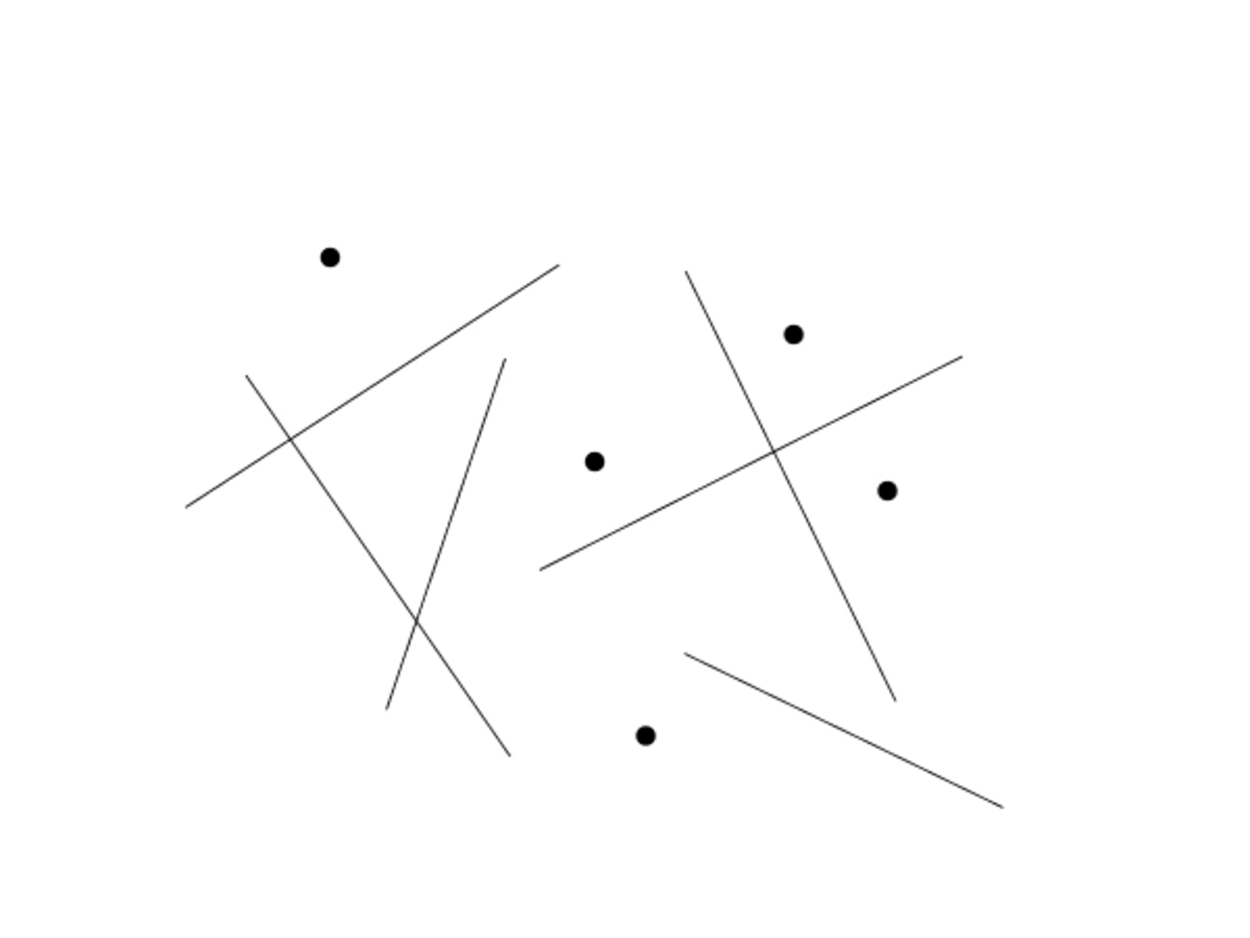
\includegraphics[width=1.5\columnwidth]{figure}
\caption{Using \texttt{figure*}, the figure spans two columns. Captions should be placed below the figure, exactly like this.
\label{fig:example}}
\end{figure*}

\subsection{Equations}
Equations of importance, or to which you refer later,
should be placed on separated lines and numbered.
The number should be on the right, between parentheses (LateX will do it for you):

\begin{equation}
E=mc^{2+\delta}.
\label{eq:Emc2}
\end{equation}

Refer to equations like so:
As (\ref{eq:Emc2}) shows, 
I do not completely trust Special Relativity.

\subsection{Figures, Tables and Captions}

\begin{table}[ht!]  % recommented placement insctructiosn for table
\centering 
\begin{tabular}{|l|l|}
  \hline
  String value & Numeric value \\
  \hline
  Hello TENOR  & 2019 \\
  \hline
 \end{tabular}
 \caption{Table captions placed below the table.}
 \label{tab:example}
\end{table}

All artwork must be centered, neat, clean, and legible. 
All lines should be very dark for purposes of reproduction and artwork should not be hand-drawn. The proceedings will be distributed in electronic form only, therefore color figures are allowed.
However, you may want to check that your figures are understandable even if they are printed in black-and-white. 
Vectorial figures are preferred. 
In order to optimize readability, the font size of text within a figure should be at least identical to footnote font size (8pt). 
If bitmap figures are used, please make sure that the resolution is enough for print quality. 

Figure and tables are numbered consecutively. Place tables/figures in text as close to the reference as possible, and preferably at the top of the page. Inline insertion of figures is preferred. Beware of the overall text and columns formatting when placing figures, in order to avoid blank space at the bottom of columns. 
Figures and tables may extend across both columns to a maximum width of 17.2cm.

Numbers and captions of figures and tables always ap-pear below the figure/table. Figure and table captions must follow the model below, with 10pt Times font, bold face for figure/table label and number, and a small spat of 3pt before and after. Captions must be justified on the whole column width if composed of several lines, of centered in case of a single line. 
In principle \LaTeX{} will deal with most of these issues for you.

\textbf{All figures and tables must be referred to in the main text body}, for example: see Figure~\ref{fig:example} and Table~\ref{fig:example} (not Fig.~\ref{fig:example}, or figure~\ref{fig:example}). 


%\begin{figure}[t]
%\figbox{
%\subfloat[][]{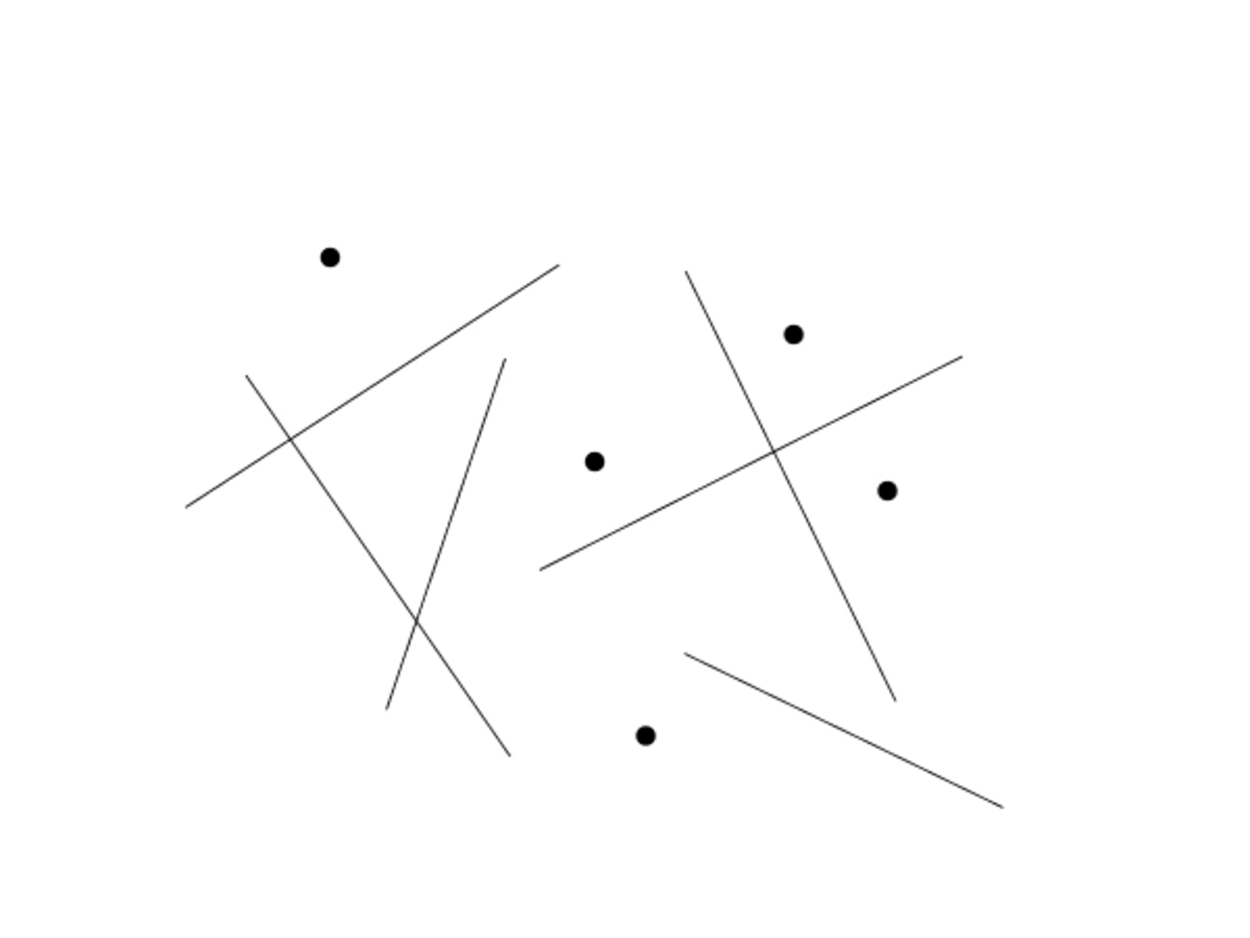
\includegraphics[width=60mm]{figure}\label{fig:subfigex_a}}\\
%\subfloat[][]{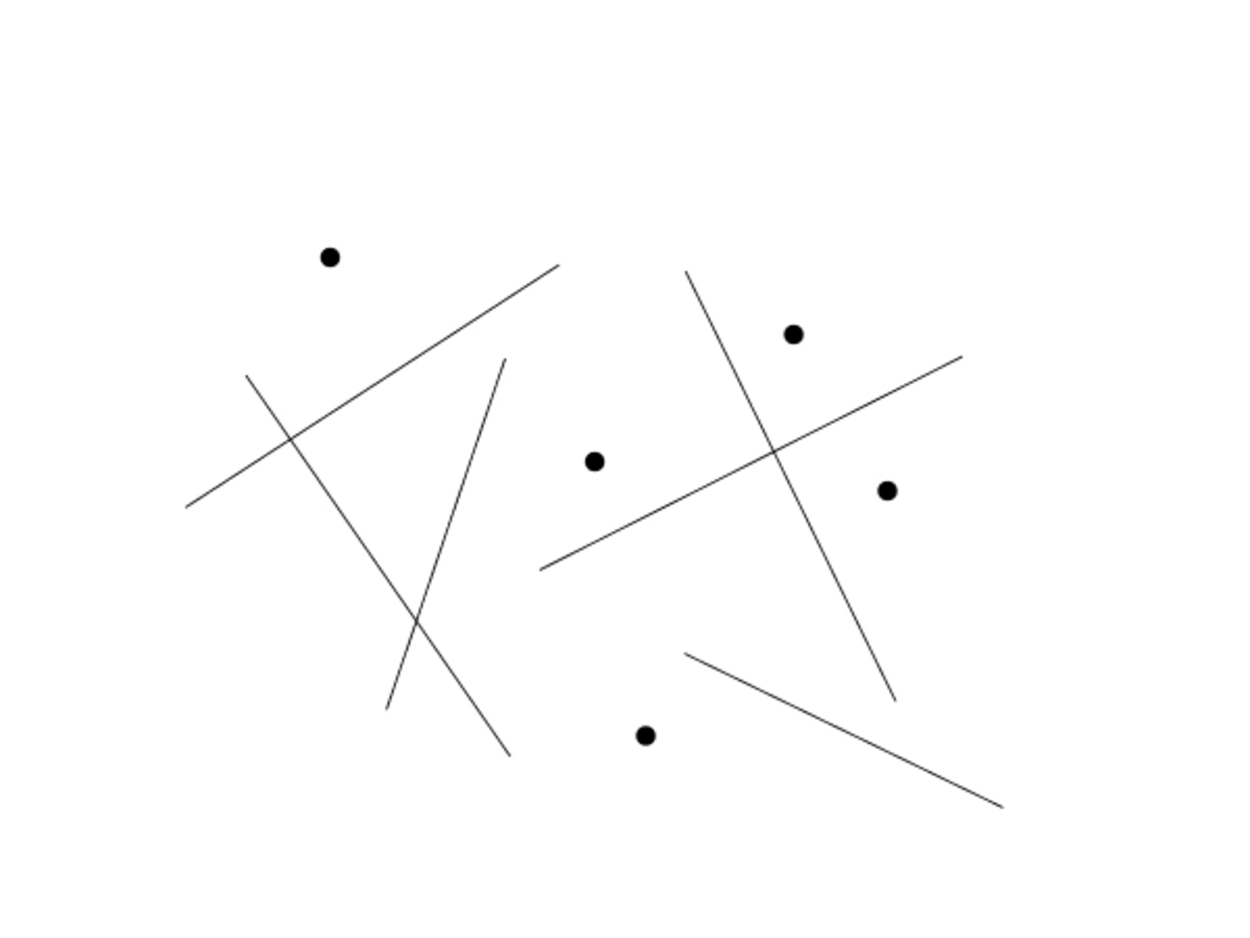
\includegraphics[width=80mm]{figure}\label{fig:subfigex_b}}
%}
%\caption{Here's an example using the subfig package.\label{fig:subfigex} }
%\end{figure}



\section{Citations}

All bibliographical references should be listed at the end, inside a numbered, first-level heading section titled REFERENCES.
References must be numbered in order of appearance. 
Reference numbers in the text should appear within square brackets, such as in~\cite{Someone:13} or~\cite{Someone:13,Someone:04,Someone:09}.
BibTeX will also handle this for you~\cite{ref:4,ref:online}.
Do not list references that do not appear in the text. 

Use references preferably for bibliographic items. Prefer footnotes to cite URLs.\footnote{My URL: http://tenor-conference.org/} 



\section{Conclusions}
To finish your full-length paper, end it with a conclusion; 
and after careful editing and a final spell-cheek,
submit it through the conference Submission System (see call for papers). 
\underline{Do not} send papers directly by e-mail.


\begin{acknowledgments}
At the end of the Conclusions, acknowledgements to people, projects, funding agencies, etc. can be included using the ``acknowledgments'' environment (similar to second-level heading, with no numbering).
\end{acknowledgments} 

%%%%%%%%%%%%%%%%%%%%%%%%%%%%%%%%%%%%%%%%%%%%%%%%%%%%%%%%%%%%%%%%%%%%%%%%%%%%%
%bibliography here
\balance % balance the columns on the last page

% use bibtex to generate the bibliography
\bibliography{tenor-template}

\end{document}
